\documentclass[12pt]{article} 
% Custom definitions
% To use this customization file, insert the line "% Custom definitions
% To use this customization file, insert the line "% Custom definitions
% To use this customization file, insert the line "\input{custom}" in the header of the tex file.

% Formatting

\tolerance=1000

% Packages

% \usepackage{amssymb,latexsym}
\usepackage{amssymb,amsfonts,amsmath,latexsym,amsthm}
\usepackage[usenames,dvipsnames]{color}
\usepackage[]{graphicx}
\usepackage[space]{grffile}
\usepackage{mathrsfs}   % fancy math font
% \usepackage[font=small,skip=0pt]{caption}
\usepackage[skip=0pt]{caption}
\usepackage{subcaption}
\usepackage{verbatim}
\usepackage{url}
\usepackage{bm}
\usepackage{dsfont}
\usepackage{extarrows}
\usepackage{multirow}
% \usepackage{wrapfig}
% \usepackage{epstopdf}
\usepackage{rotating}
\usepackage{tikz}
\usetikzlibrary{fit}					% fitting shapes to coordinates
%\usetikzlibrary{backgrounds}	% drawing the background after the foreground

% \usepackage[dvipdfm,colorlinks,citecolor=blue,linkcolor=blue,urlcolor=blue]{hyperref}
\usepackage[colorlinks,citecolor=blue,linkcolor=blue,urlcolor=blue]{hyperref}
%\usepackage{hyperref}
\usepackage[authoryear,round]{natbib}


%  Theorems, etc.

\theoremstyle{plain}
\newtheorem{theorem}{Theorem}[section]
\newtheorem{corollary}[theorem]{Corollary}
\newtheorem{lemma}[theorem]{Lemma}
\newtheorem{proposition}[theorem]{Proposition}
\newtheorem{condition}[theorem]{Condition}
% \newtheorem{conditions}[theorem]{Conditions}

\theoremstyle{definition}
\newtheorem{definition}[theorem]{Definition}
% \newtheorem*{unnumbered-definition}{Definition}
\newtheorem{example}[theorem]{Example}
\theoremstyle{remark}
\newtheorem*{remark}{Remark}
\numberwithin{equation}{section}


% footnote without number
\newcommand\blankfootnote[1]{%
  \begingroup
  \renewcommand\thefootnote{}\footnote{#1}%
  \addtocounter{footnote}{-1}%
  \endgroup
}
\makeatletter
\renewcommand\footnoterule{%
  \kern-3\p@
  \hrule\@width \textwidth
  \kern2.6\p@}
\makeatother

% Document-specific shortcuts
\newcommand{\btheta}{{\bm\theta}}
\newcommand{\bbtheta}{{\pmb{\bm\theta}}}

\newcommand{\commentary}[1]{\ifx\showcommentary\undefined\else \emph{#1}\fi}

\newcommand{\term}[1]{\textit{\textbf{#1}}}

% Math shortcuts

% Probability distributions
\DeclareMathOperator*{\Exp}{Exp}
\DeclareMathOperator*{\TExp}{TExp}
\DeclareMathOperator*{\Bernoulli}{Bernoulli}
\DeclareMathOperator*{\Beta}{Beta}
\DeclareMathOperator*{\Ga}{Gamma}
\DeclareMathOperator*{\TGamma}{TGamma}
\DeclareMathOperator*{\Poisson}{Poisson}
\DeclareMathOperator*{\Binomial}{Binomial}
\DeclareMathOperator*{\NormalGamma}{NormalGamma}
\DeclareMathOperator*{\InvGamma}{InvGamma}
\DeclareMathOperator*{\Cauchy}{Cauchy}
\DeclareMathOperator*{\Uniform}{Uniform}
\DeclareMathOperator*{\Gumbel}{Gumbel}
\DeclareMathOperator*{\Pareto}{Pareto}
\DeclareMathOperator*{\Mono}{Mono}
\DeclareMathOperator*{\Geometric}{Geometric}
\DeclareMathOperator*{\Wishart}{Wishart}

% Math operators
\DeclareMathOperator*{\argmin}{argmin}
\DeclareMathOperator*{\argmax}{argmax}
\DeclareMathOperator*{\Cov}{Cov}
\DeclareMathOperator*{\diag}{diag}
\DeclareMathOperator*{\median}{median}
\DeclareMathOperator*{\Vol}{Vol}
\newcommand{\logit}{\mathrm{logit}}

% Math characters
\newcommand{\R}{\mathbb{R}}
\newcommand{\Z}{\mathbb{Z}}
\newcommand{\E}{\mathbb{E}}
\renewcommand{\Pr}{\mathbb{P}}
\newcommand{\1}{\mathds{1}}
\newcommand{\V}{\mathbb{V}}

\newcommand{\A}{\mathcal{A}}
\newcommand{\C}{\mathcal{C}}
\newcommand{\D}{\mathcal{D}}
\newcommand{\Hcal}{\mathcal{H}}
\newcommand{\I}{\mathcal{I}}
\newcommand{\J}{\mathcal{J}}
\newcommand{\M}{\mathcal{M}}
\newcommand{\N}{\mathcal{N}}
\newcommand{\X}{\mathcal{X}}
\newcommand{\Zcal}{\mathcal{Z}}
\renewcommand{\P}{\mathcal{P}}

\newcommand{\T}{\mathtt{T}}
\renewcommand{\emptyset}{\varnothing}


% Miscellaneous commands
\newcommand{\iid}{\stackrel{\mathrm{iid}}{\sim}}
\newcommand{\matrixsmall}[1]{\bigl(\begin{smallmatrix}#1\end{smallmatrix} \bigr)}

\newcommand{\items}[1]{\begin{itemize} #1 \end{itemize}}

\newcommand{\todo}[1]{\emph{\textcolor{red}{(#1)}}}

\newcommand{\branch}[4]{
\left\{
	\begin{array}{ll}
		#1  & \mbox{if } #2 \\
		#3 & \mbox{if } #4
	\end{array}
\right.
}

% approximately proportional to
\def\app#1#2{%
  \mathrel{%
    \setbox0=\hbox{$#1\sim$}%
    \setbox2=\hbox{%
      \rlap{\hbox{$#1\propto$}}%
      \lower1.3\ht0\box0%
    }%
    \raise0.25\ht2\box2%
  }%
}
\def\approxprop{\mathpalette\app\relax}

% \newcommand{\approptoinn}[2]{\mathrel{\vcenter{
  % \offinterlineskip\halign{\hfil$##$\cr
    % #1\propto\cr\noalign{\kern2pt}#1\sim\cr\noalign{\kern-2pt}}}}}

% \newcommand{\approxpropto}{\mathpalette\approptoinn\relax}





" in the header of the tex file.

% Formatting

\tolerance=1000

% Packages

% \usepackage{amssymb,latexsym}
\usepackage{amssymb,amsfonts,amsmath,latexsym,amsthm}
\usepackage[usenames,dvipsnames]{color}
\usepackage[]{graphicx}
\usepackage[space]{grffile}
\usepackage{mathrsfs}   % fancy math font
% \usepackage[font=small,skip=0pt]{caption}
\usepackage[skip=0pt]{caption}
\usepackage{subcaption}
\usepackage{verbatim}
\usepackage{url}
\usepackage{bm}
\usepackage{dsfont}
\usepackage{extarrows}
\usepackage{multirow}
% \usepackage{wrapfig}
% \usepackage{epstopdf}
\usepackage{rotating}
\usepackage{tikz}
\usetikzlibrary{fit}					% fitting shapes to coordinates
%\usetikzlibrary{backgrounds}	% drawing the background after the foreground

% \usepackage[dvipdfm,colorlinks,citecolor=blue,linkcolor=blue,urlcolor=blue]{hyperref}
\usepackage[colorlinks,citecolor=blue,linkcolor=blue,urlcolor=blue]{hyperref}
%\usepackage{hyperref}
\usepackage[authoryear,round]{natbib}


%  Theorems, etc.

\theoremstyle{plain}
\newtheorem{theorem}{Theorem}[section]
\newtheorem{corollary}[theorem]{Corollary}
\newtheorem{lemma}[theorem]{Lemma}
\newtheorem{proposition}[theorem]{Proposition}
\newtheorem{condition}[theorem]{Condition}
% \newtheorem{conditions}[theorem]{Conditions}

\theoremstyle{definition}
\newtheorem{definition}[theorem]{Definition}
% \newtheorem*{unnumbered-definition}{Definition}
\newtheorem{example}[theorem]{Example}
\theoremstyle{remark}
\newtheorem*{remark}{Remark}
\numberwithin{equation}{section}


% footnote without number
\newcommand\blankfootnote[1]{%
  \begingroup
  \renewcommand\thefootnote{}\footnote{#1}%
  \addtocounter{footnote}{-1}%
  \endgroup
}
\makeatletter
\renewcommand\footnoterule{%
  \kern-3\p@
  \hrule\@width \textwidth
  \kern2.6\p@}
\makeatother

% Document-specific shortcuts
\newcommand{\btheta}{{\bm\theta}}
\newcommand{\bbtheta}{{\pmb{\bm\theta}}}

\newcommand{\commentary}[1]{\ifx\showcommentary\undefined\else \emph{#1}\fi}

\newcommand{\term}[1]{\textit{\textbf{#1}}}

% Math shortcuts

% Probability distributions
\DeclareMathOperator*{\Exp}{Exp}
\DeclareMathOperator*{\TExp}{TExp}
\DeclareMathOperator*{\Bernoulli}{Bernoulli}
\DeclareMathOperator*{\Beta}{Beta}
\DeclareMathOperator*{\Ga}{Gamma}
\DeclareMathOperator*{\TGamma}{TGamma}
\DeclareMathOperator*{\Poisson}{Poisson}
\DeclareMathOperator*{\Binomial}{Binomial}
\DeclareMathOperator*{\NormalGamma}{NormalGamma}
\DeclareMathOperator*{\InvGamma}{InvGamma}
\DeclareMathOperator*{\Cauchy}{Cauchy}
\DeclareMathOperator*{\Uniform}{Uniform}
\DeclareMathOperator*{\Gumbel}{Gumbel}
\DeclareMathOperator*{\Pareto}{Pareto}
\DeclareMathOperator*{\Mono}{Mono}
\DeclareMathOperator*{\Geometric}{Geometric}
\DeclareMathOperator*{\Wishart}{Wishart}

% Math operators
\DeclareMathOperator*{\argmin}{argmin}
\DeclareMathOperator*{\argmax}{argmax}
\DeclareMathOperator*{\Cov}{Cov}
\DeclareMathOperator*{\diag}{diag}
\DeclareMathOperator*{\median}{median}
\DeclareMathOperator*{\Vol}{Vol}
\newcommand{\logit}{\mathrm{logit}}

% Math characters
\newcommand{\R}{\mathbb{R}}
\newcommand{\Z}{\mathbb{Z}}
\newcommand{\E}{\mathbb{E}}
\renewcommand{\Pr}{\mathbb{P}}
\newcommand{\1}{\mathds{1}}
\newcommand{\V}{\mathbb{V}}

\newcommand{\A}{\mathcal{A}}
\newcommand{\C}{\mathcal{C}}
\newcommand{\D}{\mathcal{D}}
\newcommand{\Hcal}{\mathcal{H}}
\newcommand{\I}{\mathcal{I}}
\newcommand{\J}{\mathcal{J}}
\newcommand{\M}{\mathcal{M}}
\newcommand{\N}{\mathcal{N}}
\newcommand{\X}{\mathcal{X}}
\newcommand{\Zcal}{\mathcal{Z}}
\renewcommand{\P}{\mathcal{P}}

\newcommand{\T}{\mathtt{T}}
\renewcommand{\emptyset}{\varnothing}


% Miscellaneous commands
\newcommand{\iid}{\stackrel{\mathrm{iid}}{\sim}}
\newcommand{\matrixsmall}[1]{\bigl(\begin{smallmatrix}#1\end{smallmatrix} \bigr)}

\newcommand{\items}[1]{\begin{itemize} #1 \end{itemize}}

\newcommand{\todo}[1]{\emph{\textcolor{red}{(#1)}}}

\newcommand{\branch}[4]{
\left\{
	\begin{array}{ll}
		#1  & \mbox{if } #2 \\
		#3 & \mbox{if } #4
	\end{array}
\right.
}

% approximately proportional to
\def\app#1#2{%
  \mathrel{%
    \setbox0=\hbox{$#1\sim$}%
    \setbox2=\hbox{%
      \rlap{\hbox{$#1\propto$}}%
      \lower1.3\ht0\box0%
    }%
    \raise0.25\ht2\box2%
  }%
}
\def\approxprop{\mathpalette\app\relax}

% \newcommand{\approptoinn}[2]{\mathrel{\vcenter{
  % \offinterlineskip\halign{\hfil$##$\cr
    % #1\propto\cr\noalign{\kern2pt}#1\sim\cr\noalign{\kern-2pt}}}}}

% \newcommand{\approxpropto}{\mathpalette\approptoinn\relax}





" in the header of the tex file.

% Formatting

\tolerance=1000

% Packages

% \usepackage{amssymb,latexsym}
\usepackage{amssymb,amsfonts,amsmath,latexsym,amsthm}
\usepackage[usenames,dvipsnames]{color}
\usepackage[]{graphicx}
\usepackage[space]{grffile}
\usepackage{mathrsfs}   % fancy math font
% \usepackage[font=small,skip=0pt]{caption}
\usepackage[skip=0pt]{caption}
\usepackage{subcaption}
\usepackage{verbatim}
\usepackage{url}
\usepackage{bm}
\usepackage{dsfont}
\usepackage{extarrows}
\usepackage{multirow}
% \usepackage{wrapfig}
% \usepackage{epstopdf}
\usepackage{rotating}
\usepackage{tikz}
\usetikzlibrary{fit}					% fitting shapes to coordinates
%\usetikzlibrary{backgrounds}	% drawing the background after the foreground

% \usepackage[dvipdfm,colorlinks,citecolor=blue,linkcolor=blue,urlcolor=blue]{hyperref}
\usepackage[colorlinks,citecolor=blue,linkcolor=blue,urlcolor=blue]{hyperref}
%\usepackage{hyperref}
\usepackage[authoryear,round]{natbib}


%  Theorems, etc.

\theoremstyle{plain}
\newtheorem{theorem}{Theorem}[section]
\newtheorem{corollary}[theorem]{Corollary}
\newtheorem{lemma}[theorem]{Lemma}
\newtheorem{proposition}[theorem]{Proposition}
\newtheorem{condition}[theorem]{Condition}
% \newtheorem{conditions}[theorem]{Conditions}

\theoremstyle{definition}
\newtheorem{definition}[theorem]{Definition}
% \newtheorem*{unnumbered-definition}{Definition}
\newtheorem{example}[theorem]{Example}
\theoremstyle{remark}
\newtheorem*{remark}{Remark}
\numberwithin{equation}{section}


% footnote without number
\newcommand\blankfootnote[1]{%
  \begingroup
  \renewcommand\thefootnote{}\footnote{#1}%
  \addtocounter{footnote}{-1}%
  \endgroup
}
\makeatletter
\renewcommand\footnoterule{%
  \kern-3\p@
  \hrule\@width \textwidth
  \kern2.6\p@}
\makeatother

% Document-specific shortcuts
\newcommand{\btheta}{{\bm\theta}}
\newcommand{\bbtheta}{{\pmb{\bm\theta}}}

\newcommand{\commentary}[1]{\ifx\showcommentary\undefined\else \emph{#1}\fi}

\newcommand{\term}[1]{\textit{\textbf{#1}}}

% Math shortcuts

% Probability distributions
\DeclareMathOperator*{\Exp}{Exp}
\DeclareMathOperator*{\TExp}{TExp}
\DeclareMathOperator*{\Bernoulli}{Bernoulli}
\DeclareMathOperator*{\Beta}{Beta}
\DeclareMathOperator*{\Ga}{Gamma}
\DeclareMathOperator*{\TGamma}{TGamma}
\DeclareMathOperator*{\Poisson}{Poisson}
\DeclareMathOperator*{\Binomial}{Binomial}
\DeclareMathOperator*{\NormalGamma}{NormalGamma}
\DeclareMathOperator*{\InvGamma}{InvGamma}
\DeclareMathOperator*{\Cauchy}{Cauchy}
\DeclareMathOperator*{\Uniform}{Uniform}
\DeclareMathOperator*{\Gumbel}{Gumbel}
\DeclareMathOperator*{\Pareto}{Pareto}
\DeclareMathOperator*{\Mono}{Mono}
\DeclareMathOperator*{\Geometric}{Geometric}
\DeclareMathOperator*{\Wishart}{Wishart}

% Math operators
\DeclareMathOperator*{\argmin}{argmin}
\DeclareMathOperator*{\argmax}{argmax}
\DeclareMathOperator*{\Cov}{Cov}
\DeclareMathOperator*{\diag}{diag}
\DeclareMathOperator*{\median}{median}
\DeclareMathOperator*{\Vol}{Vol}
\newcommand{\logit}{\mathrm{logit}}

% Math characters
\newcommand{\R}{\mathbb{R}}
\newcommand{\Z}{\mathbb{Z}}
\newcommand{\E}{\mathbb{E}}
\renewcommand{\Pr}{\mathbb{P}}
\newcommand{\1}{\mathds{1}}
\newcommand{\V}{\mathbb{V}}

\newcommand{\A}{\mathcal{A}}
\newcommand{\C}{\mathcal{C}}
\newcommand{\D}{\mathcal{D}}
\newcommand{\Hcal}{\mathcal{H}}
\newcommand{\I}{\mathcal{I}}
\newcommand{\J}{\mathcal{J}}
\newcommand{\M}{\mathcal{M}}
\newcommand{\N}{\mathcal{N}}
\newcommand{\X}{\mathcal{X}}
\newcommand{\Zcal}{\mathcal{Z}}
\renewcommand{\P}{\mathcal{P}}

\newcommand{\T}{\mathtt{T}}
\renewcommand{\emptyset}{\varnothing}


% Miscellaneous commands
\newcommand{\iid}{\stackrel{\mathrm{iid}}{\sim}}
\newcommand{\matrixsmall}[1]{\bigl(\begin{smallmatrix}#1\end{smallmatrix} \bigr)}

\newcommand{\items}[1]{\begin{itemize} #1 \end{itemize}}

\newcommand{\todo}[1]{\emph{\textcolor{red}{(#1)}}}

\newcommand{\branch}[4]{
\left\{
	\begin{array}{ll}
		#1  & \mbox{if } #2 \\
		#3 & \mbox{if } #4
	\end{array}
\right.
}

% approximately proportional to
\def\app#1#2{%
  \mathrel{%
    \setbox0=\hbox{$#1\sim$}%
    \setbox2=\hbox{%
      \rlap{\hbox{$#1\propto$}}%
      \lower1.3\ht0\box0%
    }%
    \raise0.25\ht2\box2%
  }%
}
\def\approxprop{\mathpalette\app\relax}

% \newcommand{\approptoinn}[2]{\mathrel{\vcenter{
  % \offinterlineskip\halign{\hfil$##$\cr
    % #1\propto\cr\noalign{\kern2pt}#1\sim\cr\noalign{\kern-2pt}}}}}

% \newcommand{\approxpropto}{\mathpalette\approptoinn\relax}







\usepackage[authoryear,round]{natbib}
\usepackage{multirow}
\usepackage{mathtools}

\usetikzlibrary{fit}                    % fitting shapes to coordinates
\usetikzlibrary{backgrounds}    % drawing the background after the foreground


\title{Homework: Variational inference for population structure mixture models}
\author{}
\date{}


\begin{document}
\maketitle

\thispagestyle{firststyle}


\vspace{2em}



\section{Background}

In a large number of biology applications, the data consist of measurements from a number of organisms, and it is important to understand the ``population structure'' exhibited by these organisms.  Organisms tend to segregate into populations, such that individuals within a given population interbreed commonly, while breeding between populations is much less common.  This causes the data to tend to fall into clusters corresponding to these populations. It is important to infer these clusters and take them into account for many types of analysis.  Failure to account for population structure can lead to misleading results, due to Simpson's paradox.
The standard way to infer population structure from genotype data is to use what is called an ``admixture model''.  We will consider a simplification based on an ordinary mixture model.  The article introducing these models \citep{pritchard2000inference} is one of the most highly cited statistics papers of all time, with 16,498 citations as of this writing, according to Google Scholar.


\section{Data}

We will consider data from \citet{lorenzen2004no} and \citet{lorenzen2006regional}, consisting of genotypes from $n = 216$ common impala and black-faced impala from Southern Africa (see Figure \ref{figure:impala}).  The common impala is widespread throughout the eastern part of Southern Africa, whereas the black-faced impala is an endangered subspecies that is localized to a small region in the western part. These researchers were interested in understanding the genetic diversity of these animals, in order to help save the black-faced impala from extinction.

For each animal $j = 1,\ldots,n$, its genotype was determined at $L = 8$ loci (i.e., $8$ locations on the genome). At each locus $\ell = 1,\ldots,8$, the genotype of animal $j$ consists of two allele copies, $x_{j \ell 1},x_{j \ell 2} \in \{1,\ldots,V_\ell \}$ (since each animal has two copies of each chromosome, one from each parent). Here, $V_\ell$ is the number of different variants of allele copy that can occur at locus $\ell$, and for this data set, $V = (15,13,6,6,9,14,16,9)$. For example, Table \ref{table:example} shows the data for animal $j = 86$. Missing entries are indicated by $-1$. The file ``x.txt'' contains the genotype data for all $n = 216$ animals.





\begin{figure}
\begin{center}
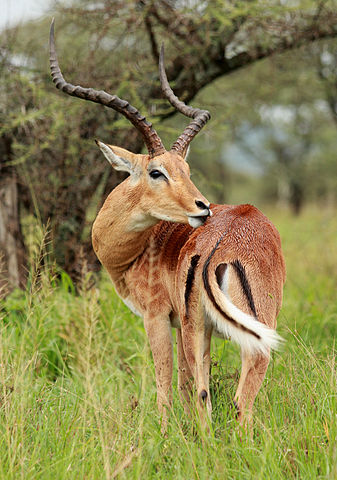
\includegraphics[height=.2\textheight]{figures/common-impala.jpg}
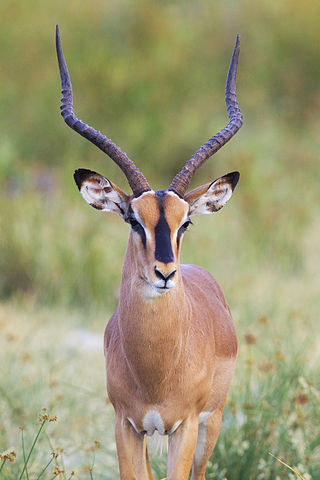
\includegraphics[height=.2\textheight]{figures/black-faced-impala.jpg}
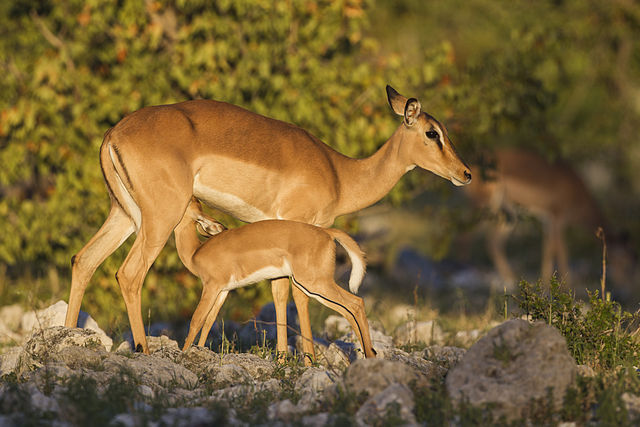
\includegraphics[height=.2\textheight]{figures/female-impala.jpg}
\end{center}
\caption[]{Left: Male common impala. Middle: Male black-faced impala. Right: Female and offspring black-faced impala.\footnotemark}
\label{figure:impala}
\end{figure}

\footnotetext{Image credits:
Common impala,
\href{https://commons.wikimedia.org/wiki/File:ImpalaSerengetiNationalParkMar2011.jpg}{Filip Lachowski, CC BY-SA 2.0}.
Black-faced impala,
\href{https://commons.wikimedia.org/wiki/File:Black-faced_impala_from_Etosha_National_Park,_Namibia,_2014.jpg}{Yathin S Krishnappa, CC BY-SA 3.0}.
Female and offspring,
\href{https://commons.wikimedia.org/wiki/File:Aepyceros_melampus_petersi_-_Etosha_2014.jpg}{Yathin S Krishnappa, CC BY-SA 3.0}.
}


\begin{table}
\centering
\caption{Genotype of animal $j = 86$}%
\label{table:example}%
\begin{tabular}{|l|c|c|c|c|c|c|c|c|c|c|c|c|c|c|c|c|}%
\hline
Locus $\ell$ & 
\multicolumn{2}{|c|}{1} & 
\multicolumn{2}{|c|}{2} &
\multicolumn{2}{|c|}{3} & 
\multicolumn{2}{|c|}{4} &
\multicolumn{2}{|c|}{5} & 
\multicolumn{2}{|c|}{6} &
\multicolumn{2}{|c|}{7} & 
\multicolumn{2}{|c|}{8} \\
\hline
Allele copy $c$ & 1 & 2 & 1 & 2 & 1 & 2 & 1 & 2 & 1 & 2 & 1 & 2 & 1 & 2 & 1 & 2 \\
\hline
Variant observed, $x_{j \ell c}$ 
& 5 & 3  &  2 & 2  & -1 & -1  & 2 & 2 &  1 & 2 &  3 & 6  & 3 & 2  & 1 & 1\\   
%& 1 & 4  &  2 & 2  &  1 & 2  &  1 & 1  &  2 & 3  &  3 & 2  &  3 & 2  &  1 & 1 
\hline
\end{tabular}
\end{table}



\section{Model}

Consider the following model. Suppose there are $k$ mixture components, representing $k$ different populations. 
The component weights are $w = (w_1,\ldots,w_k)$, where $w_i \geq 0$ and $\sum_{i = 1}^k w_i = 1$. The component parameters are $\alpha =(\alpha_1,\ldots,\alpha_k)$, where for each component $i = 1,\ldots,k$,
$$\alpha_i = \begin{bmatrix*}[l] 
\alpha_{i 1}(1),\ldots,\alpha_{i 1}(V_1)\\
~~~~\vdots\\
\alpha_{i \ell}(1),\ldots,\alpha_{i \ell}(V_\ell)\\
~~~~\vdots\\
\alpha_{i L}(1),\ldots,\alpha_{i L}(V_L)
\end{bmatrix*},$$
with $\alpha_{i \ell}(v)$ being the probability of observing variant $v$ at locus $\ell$ for an animal in population $i$. Note that this is a ``ragged matrix'', i.e., the rows have different lengths. Each row $\alpha_{i \ell}$ is a probability vector, in other words, $\alpha_{i \ell}(v) \geq 0$ and $\sum_{v = 1}^{V_\ell} \alpha_{i \ell}(v) = 1$. 

The data is modeled as
\begin{align*}
& Z_j | w \,\sim\, \mathrm{Categorical}(w)\\
& X_{j \ell 1},X_{j \ell 2} \mid \alpha,\,Z_j = i \,\,\sim\,\mathrm{Categorical}(\alpha_{i\ell}) \text{ independently for $\ell=1,\ldots,L$,}
\end{align*}
independently for each $j = 1,\ldots,n$.\footnote{Technically, the allele counts at each locus should be $\mathrm{Multinomial}(2,\alpha_{i \ell})$, since the order of the two allele copies is undetermined. However, to keep the assignment from getting too complicated, we will use the simpler Categorical model.}
See Figure \ref{figure:model} for the graphical model.
We will use uniform priors on $w$ and on $\alpha_{i \ell}$ for all $i,\ell$.

\begin{figure}[ht]
\begin{center}
\tikzstyle{hidden}=[circle,
                        thick,
                        draw=black,
                        fill=white]
                        % minimum size=1.5ex,


\tikzstyle{observed}=[circle,
                        thick,
                        draw=black,
                        fill=gray!60]
                        % minimum size=1.5ex,


\tikzstyle{plate}=[rectangle,
                        draw=black,
                        fill=none,
                        inner sep=.8ex,
                        rounded corners=.6ex]

\begin{tikzpicture}[>=latex] %,text height=1.5ex,text depth=0.25ex]
  % The various elements are conveniently placed using a matrix:
  \matrix[row sep=2.5ex,column sep=2.5ex] {
        \node (w) [hidden] {\large $w$};  & 
        \node (a) [hidden] {\large $\alpha$};  \\
        \node (z) [hidden] { $Z_j$};  & 
        \node (x) [hidden] { $X_j$};
		\\
    };
    
    % The diagram elements are now connected through arrows:
    \path[->]
        (w) edge[thick] (z)
        (z) edge[thick] (x)
        (a) edge[thick] (x)
;
    \begin{pgfonlayer}{background}
        \node (myplate) [plate, fit=(x)(z)] {};
        %\node[anchor=south east,inner sep=.5ex] at (myplate.south east) {\small $j=1,\ldots,n$};
    \end{pgfonlayer}

\end{tikzpicture}
\end{center}

\caption{Directed graphical model.}
\label{figure:model}
\end{figure}

In this homework, you will construct a variational approximation to the posterior on $z,w,\alpha$ for this model. The target distribution is
\begin{align*}
\pi(z,w,\alpha) &= p(z,w,\alpha | x) \propto p(x,z,w,\alpha)
\propto p(x | z,\alpha) p(z | w)\\
& = \prod_{j = 1}^n \Big(\prod_{\ell = 1}^L \prod_{c = 1}^2 
\alpha_{z_j \ell}(x_{j \ell c}) \Big) w_{z_j}.
\end{align*}
Taking the log and using indicator functions to simplify the dependence on the parameters, we get
\begin{align*}
\log \pi(z,w,\alpha) = \sum_{j = 1}^n \sum_{i = 1}^k
\1(z_j = i) \Big(\log w_i + \sum_{\ell = 1}^L \sum_{c = 1}^2 \sum_{v = 1}^{V_\ell} \1(x_{j \ell c} = v) \log \alpha_{i \ell}(v)\Big) + \text{const}.
\end{align*}
To handle the missing data, let's assume the data collection process is ignorable (since the model is already complicated enough for this homework exercise).  With this assumption, the same exact expression as above can be used for $\log \pi(z,w,\alpha)$, for roughly the following reason:  in the sum over $v= 1,\ldots,V_\ell$, the indicator $\1(x_{j \ell c} = v)$ will always be zero if $x_{j \ell c}$ is missing, because $-1$ is never equal to $v$; therefore any missing data will not factor into the likelihood. Note, however, that you will need to be careful in manipulating this expression, since this means that
$ \sum_{v = 1}^{V_\ell} \1(x_{j \ell c} = v) \log \alpha_{i \ell}(v) \neq \log \alpha_{i \ell}(x_{j \ell c}) $
if $x_{j \ell c}$ is missing, because the left-hand side is zero and $\alpha_{i \ell}(-1)$ is undefined.

\section{Exercises}

\begin{enumerate}
\item Derive the variational inference algorithm for this model based on an approximating distribution of the form $q(z,w,\alpha) = q(z) q(w,\alpha)$. Hint: Similarly to the mixture model we considered in class, for the $q(z)$ update, the algorithm will involve computing $r_j(i) = \Pr_q(Z_j = i)$ (but with a different formula than before), and for the $q(w,\alpha)$ update, it will involve computing $R_i = \sum_{j = 1}^n r_j(i)$ as well as some other quantities $S_{i \ell}(v)$ that you will need to determine.

\item Implement the algorithm using a random initialization. For the convergence criterion, stop when the root-mean-square difference between $r^\text{new}$ and $r^\text{old}$ is less than $10^{-10}$, that is, when
$$\Big(\frac{1}{n k}\sum_{j = 1}^n \sum_{i = 1}^k \big(r_j^\text{new}(i) - r_j^\text{old}(i)\big)^2 \Big)^{1/2} < 10^{-10}. $$

\item Now, with $k = 4$ components, run the algorithm five times on the data in ``x.txt'', using a different random initialization each time. For each of these five runs, report the number of iterations until convergence, and plot the final values of $r_j(i)$ in a stacked bar plot as shown in Figure \ref{figure:results}. Discuss the interpretation of these plots.

\item Table \ref{table:sources} indicates the subspecies (``C'' for common impala or ``B'' for black-faced impala) and the region of origin for each animal. Do your results appear to make sense, at least roughly, in light of this additional information? Discuss. Are there any individual animals who are consistently clustered differently than other members of their subspecies and region? Give the indices $j$ of two or three animals like this, and discuss possible explanations.
\end{enumerate}

\begin{figure}
\begin{center}
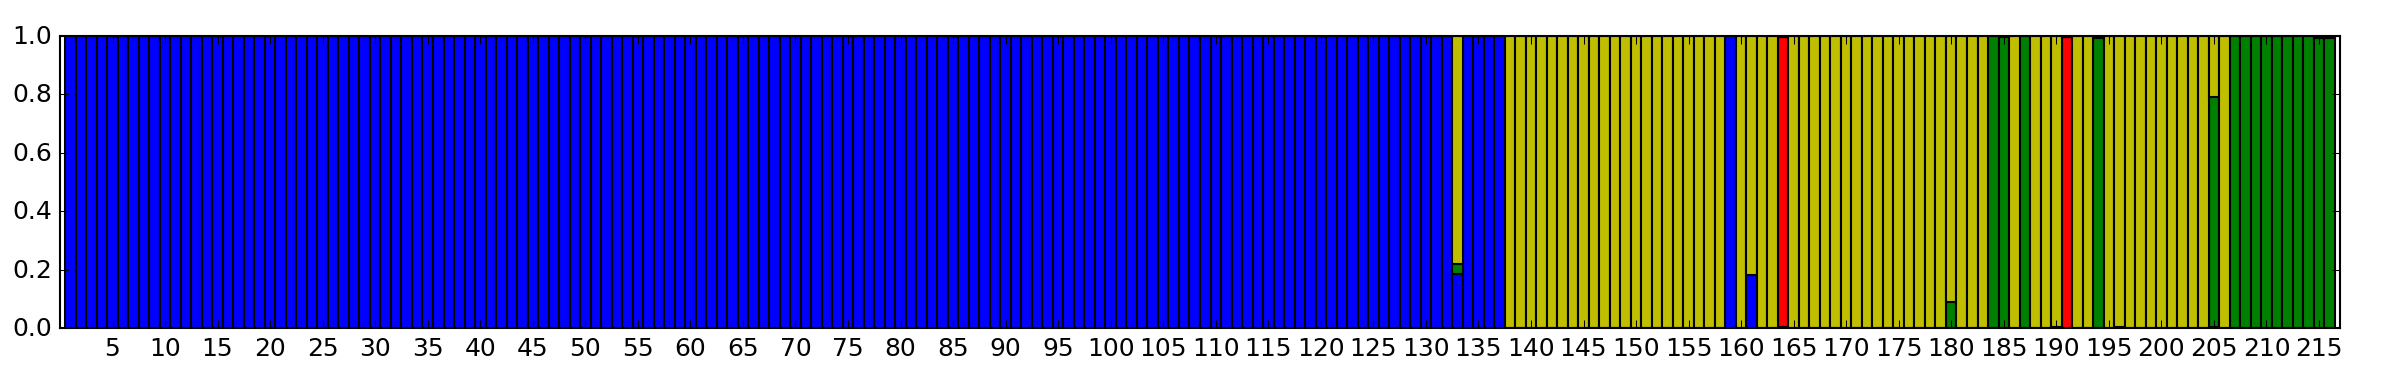
\includegraphics[width=1\textwidth]{figures/results1.png}
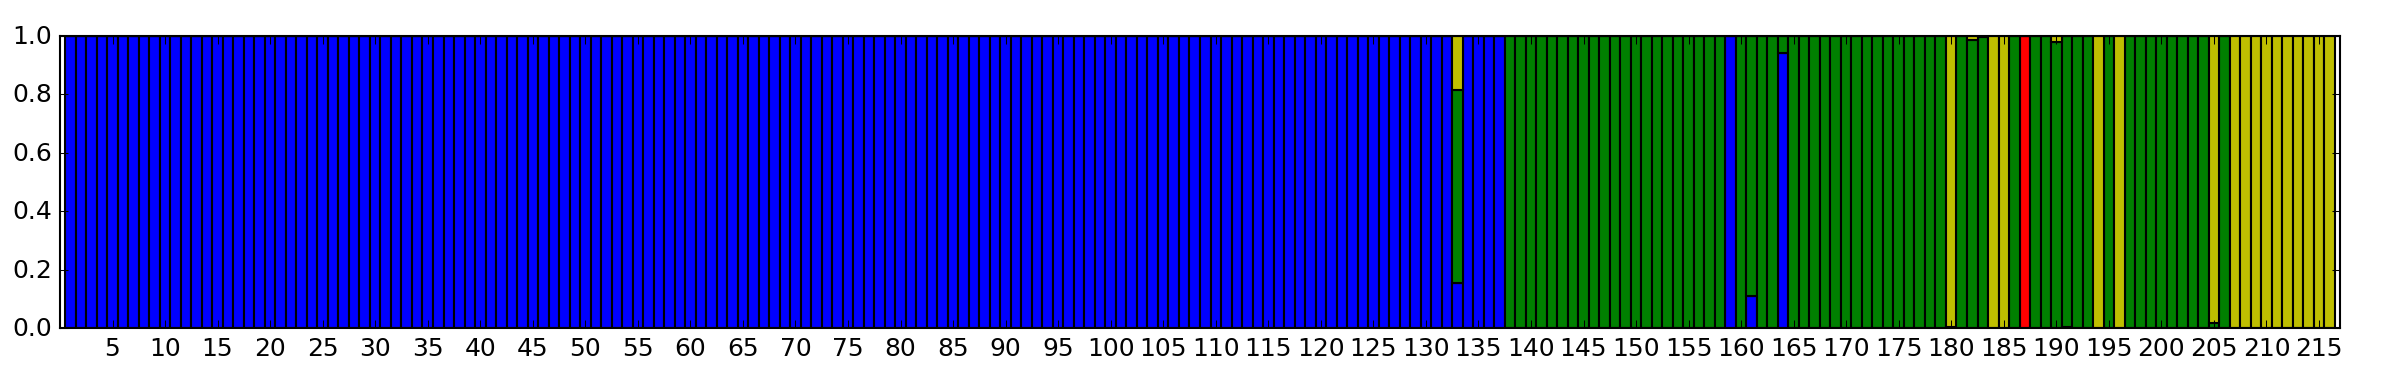
\includegraphics[width=1\textwidth]{figures/results2.png}
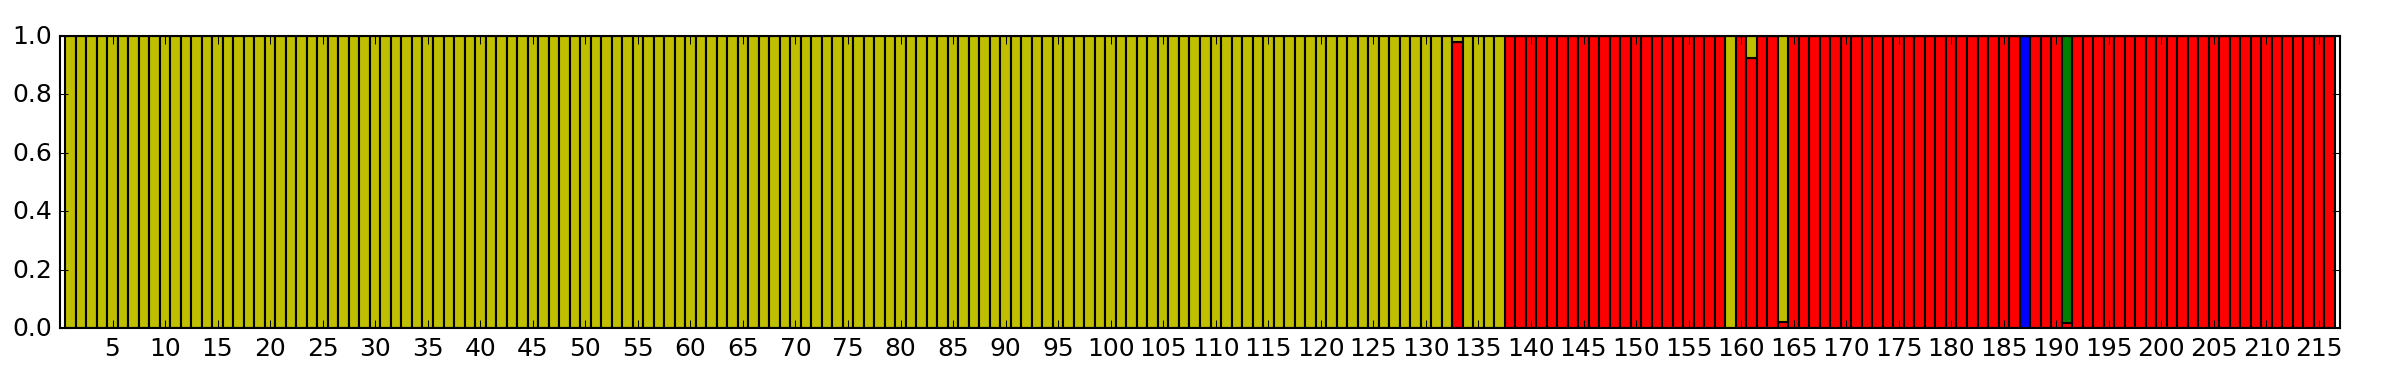
\includegraphics[width=1\textwidth]{figures/results3.png}
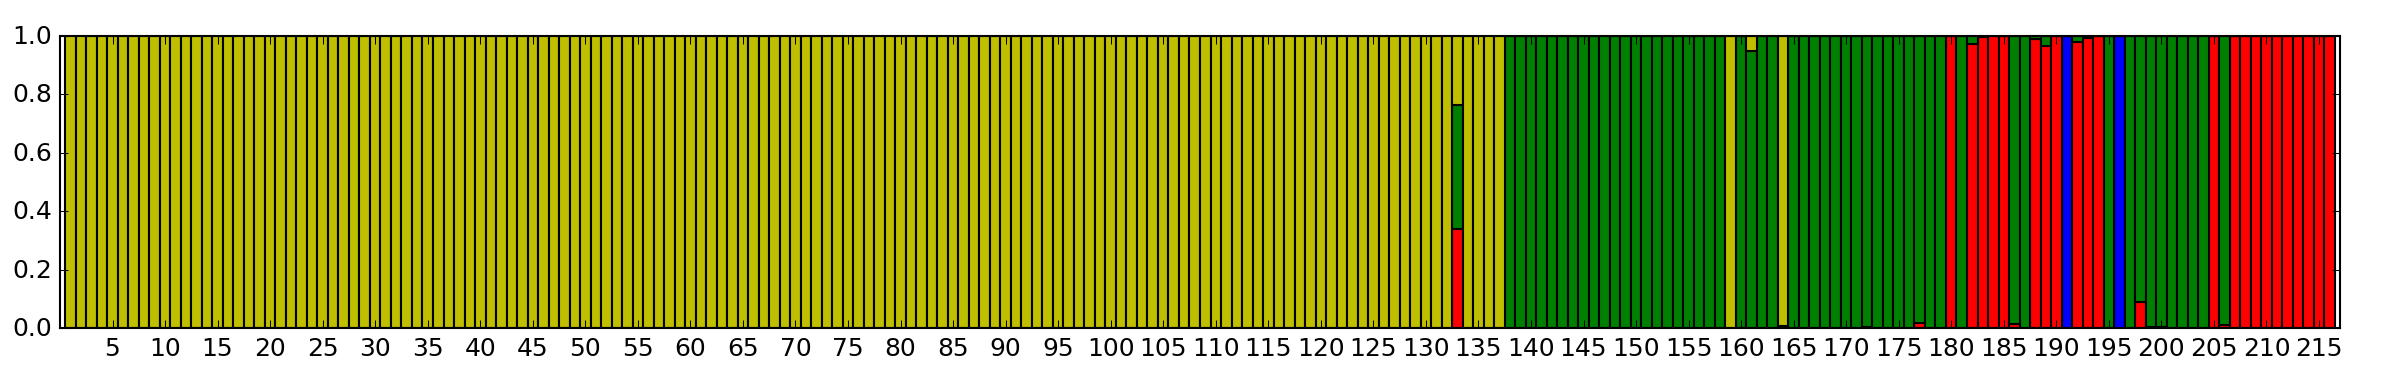
\includegraphics[width=1\textwidth]{figures/results4.png}
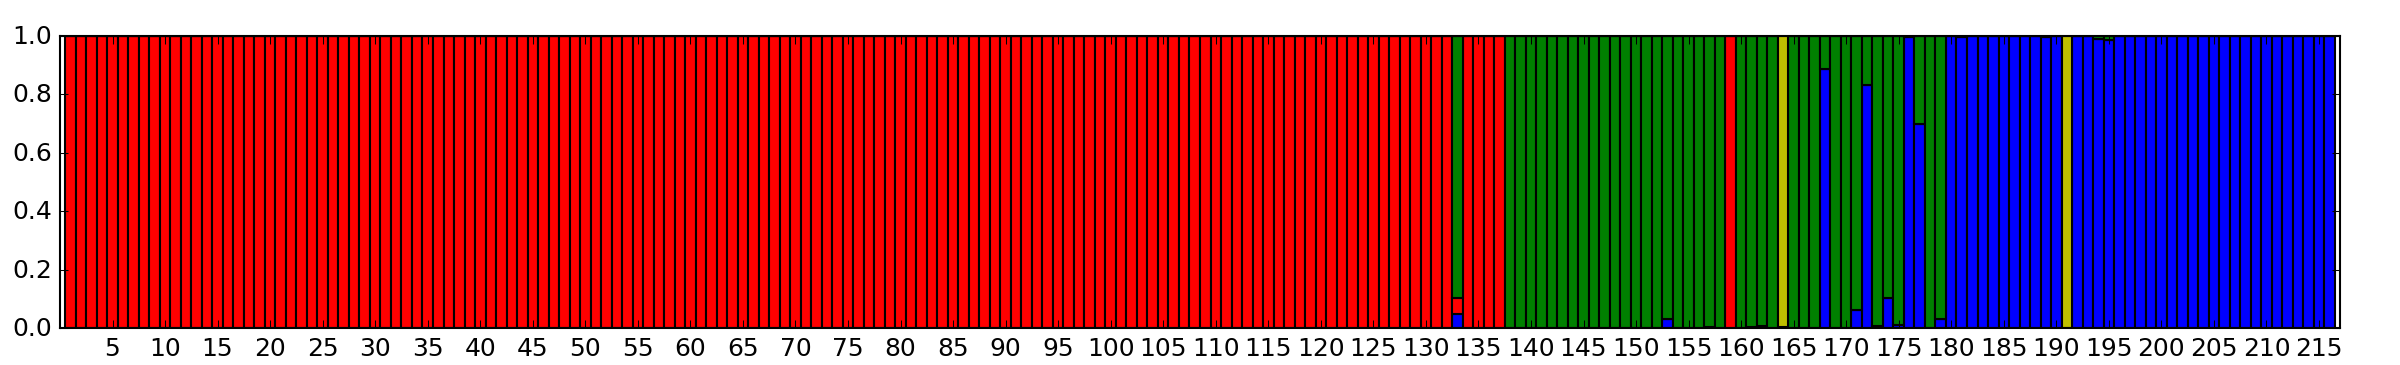
\includegraphics[width=1\textwidth]{figures/results5.png}
\end{center}
\caption{Example results from five runs with different random initializations.}
\label{figure:results}
\end{figure}


\begin{table}
\centering
\caption{Subspecies and region for each animal.}%
\label{table:sources}%
\begin{tabular}{|l|c|c|}
\hline
Animal $j$ & Subspecies & Region code \\
\hline
1-15 & B & KA \\
16-31 & B & OM \\
32-64 & B & OL \\
65-98 & B & HA \\
99-127 & B & NA \\
128-137 & B & ON \\
138-147 & C & CH\\
148-158 & C & SH\\
159-163 & C & KAF\\
164-169 & C & LU\\
170-181 & C & SE\\
182-194 & C & BU\\
195-206 & C & IM\\
207-216 & C & SA\\
\hline
\end{tabular}
\end{table}


Note that the algorithm does not converge to the same thing every time. For example, sometimes, two given animals will be assigned to the same component with very high probability in one run, but assigned to two different components with very high probability in another run. This may be because these kinds of variational approximations tend to underestimate uncertainty (in other words, they tend to be ``overconfident'').






\bibliography{refs}
\bibliographystyle{plainnat}



\end{document}

























